\begin{frame}
  \centering
  \textbf{\Large{Self-Consistent Field Methods}}
\end{frame}

\begin{frame}
  \frametitle{SCF methods}
  \centering
  \textbf{Kohn-Sham equations}
  \begin{equation}
    \nonumber
    \bigg[-\frac{1}{2}\nabla^2 + \hat{V}\bigg]\orbital_i(r) = \epsilon_i \orbital_i(r)
  \end{equation}

  \begin{itemize}
    \item How are the SCF equations usually solved?
    \item Roothaan-Hall equations
    \item Why can't we do the same with MWs?
    \item What can we do instead?
  \end{itemize}
\end{frame}

\begin{frame}
  \frametitle{One-electron systems}
  \centering
  \textbf{Schr\"{o}dinger equation}
  \begin{equation}
    \nonumber
    \bigg[-\frac{1}{2}\nabla^2 + \potential\bigg]\wavefunction(r) = E \wavefunction(r)
  \end{equation}

  \vspace{5mm}

  \textbf{Rewrite using} $\mu^2 = -2E$
  \begin{align}
    \nonumber
    \Big[-\nabla^2 + \mu^2\Big]\wavefunction(r) =&\ -2 \potential \wavefunction(r)\\
    \nonumber
    \wavefunction(r) =&-2\Big[-\nabla^2 + \mu^2\Big]^{-1} \potential \wavefunction(r)\\
    \nonumber
    \wavefunction =&-2\Helm\Big[\potential \wavefunction\Big]
  \end{align}

  \vspace{5mm}

  \textbf{Bound-State Helmholtz operator}
  \begin{equation}
    \nonumber
    \Helm f(r) = \Big[-\nabla^2 + \mu^2\Big]^{-1} f(r) = \int \frac{e^{-\mu |r-r'|}}{4\pi|r-r'|}f(r')dr'
  \end{equation}

  \vspace{5mm}

  \centering
  \tiny
  MH Kalos,
  {\it Phys. Rev.},
  \textbf{128(4)},
  1791 (1962)\\
  RJ Harrison, GI Fann, T Yanai, Z Gan and G Beylkin,
  {\it J. Chem. Phys.},
  \textbf{121},
  11587 (2004)
\end{frame}

% \begin{frame}
%   \centering
%   \textbf{\Large{Iterative solution algorithms}}
% \end{frame}

\begin{frame}
  \frametitle{Power iteration}
  \centering
  \textbf{Power iteration of the BSH operator}
  \begin{equation}
    \nonumber
    \wavefunction^{n+1} = -2\Helm^n\Big[\potential \wavefunction^n\Big]
  \end{equation}

  \vspace{3mm}

  \textbf{Finding roots of the residual}
  \begin{equation}
    \nonumber
    f(\wavefunction) = -2\Helm^n\big[\potential \wavefunction\big] - \wavefunction
  \end{equation}

  \vspace{3mm}

  \textbf{Newton's method}
  \begin{equation}
    \nonumber
    \wavefunction^{n+1} = \wavefunction^n - \Big[J(\wavefunction^n)\Big]^{-1} f(\wavefunction^n)
  \end{equation}

  \begin{equation}
  \nonumber
    \wavefunction^{n+1} = \wavefunction^n - \Big[J(\wavefunction^n)\Big]^{-1}
    \bigg(-2G^n\Big[\potential \wavefunction^n\Big] - \wavefunction^n\bigg)
  \end{equation}

  \vspace{3mm}

  So the direct power iteration is an "inexact" Newton method\\
  where we approximate the Jacobian $J(\wavefunction^n) \approx -1$.
\end{frame}

\begin{frame}
    \frametitle{Energy update}
    \centering
    \textbf{Using the relation}
    \begin{equation}
        \nonumber
        -2\hat{G}^n = \big(\hat{T} - E^n\big)^{-1}
    \end{equation}

    \vspace{5mm}

    \textbf{Manipulating the energy expression}
    \begin{align}
        \tilde{E}^{n+1}
        \nonumber
        &=	\langle\tilde{\psi}^{n+1}| \hat{T}+\hat{V} | \tilde{\psi}^{n+1}\rangle\\
        \nonumber
        &=	\langle\tilde{\psi}^{n+1}|  \hat{T} - E^n  | \tilde{\psi}^{n+1}\rangle
        +	\langle\tilde{\psi}^{n+1}|  E^n + \hat{V}  | \tilde{\psi}^{n+1}\rangle\\
        \nonumber
        &=	\langle\tilde{\psi}^{n+1}|  \hat{T} - E^n  |
	        -2\hat{G}^n\big[\hat{V}\psi^n\big]\rangle
        +	\langle\tilde{\psi}^{n+1}| E^n + \hat{V} |\tilde{\psi}^{n+1}\rangle\\
        \nonumber
        &= -\langle\tilde{\psi}^{n+1}| \hat{V} |\psi^{n}\rangle
        +	\langle\tilde{\psi}^{n+1}| E^n + \hat{V} |\tilde{\psi}^{n+1}\rangle\\
        \nonumber
        &= E^{n}\langle\tilde{\psi}^{n+1}|\tilde{\psi}^{n+1}\rangle +
	    \langle\tilde{\psi}^{n+1}| \hat{V} |\Delta\tilde{\psi}^{n}\rangle
    \end{align}

    \vspace{8mm}

    \centering
    \textbf{Energy without kinetic operator}
    \begin{equation}
        \nonumber
        E^{n+1} = E^{n} +
        \frac{\langle\tilde{\psi}^{n+1}| \hat{V} |\Delta\tilde{\psi}^{n}\rangle}
        {\langle\tilde{\psi}^{n+1}|\tilde{\psi}^{n+1}\rangle}
    \end{equation}
\end{frame}


\begin{frame}
  \frametitle{One-electron algorithm}
  \begin{columns}
    \begin{column}{.50\textwidth}
      \centering
      \textbf{Initialize BSH operator} $\Helm^n$
      \begin{equation}
        \nonumber
        \mu^n = \sqrt{-2E^n}
      \end{equation}
    \end{column}

    \begin{column}{.50\textwidth}
      \centering
      \textbf{Power iteration}
      \begin{equation}
        \nonumber
        \tilde{\wavefunction}^{n+1} = -2\Helm^n \Big[\potential \wavefunction^n \Big]
      \end{equation}
    \end{column}
  \end{columns}

  \vspace{5mm}

  \begin{columns}
    \begin{column}{.50\textwidth}
      \centering
      \textbf{Wavefunction update}
      \begin{equation}
        \nonumber
        \Delta\wavefunction^n =
        \frac{\tilde{\wavefunction}^{n+1}}{\|\tilde{\wavefunction}^{n+1}\|} - \wavefunction^n
      \end{equation}
    \end{column}

    \begin{column}{.50\textwidth}
      \centering
      \textbf{Energy update}
      \begin{equation}
        \nonumber
        \Delta E^n =
        \frac{\langle\tilde{\wavefunction}^{n+1}|\potential|\Delta\tilde{\wavefunction}^n\rangle}
        {\langle\tilde{\wavefunction}^{n+1}|\tilde{\wavefunction}^{n+1}\rangle}
      \end{equation}
    \end{column}
  \end{columns}

  \vspace{10mm}

  \centering
  \textbf{Update wavefunction and energy}
  \begin{align}
    \nonumber
    \wavefunction^{n+1} &= \wavefunction^n + \Delta \wavefunction^n\\
    \nonumber
    E^{n+1} &= E^n + \Delta E^n
  \end{align}
\end{frame}

\begin{frame}
  \frametitle{Hydrogen atom}
  \begin{itemize}
    \item Hydrogen potential
    \item Hydrogen integral equation
    \item Hydrogen energy update
    \item Power iteration convergence plot
  \end{itemize}
\end{frame}

% \begin{frame}
%   \frametitle{One-electron systems}
%   \centering
%   \textbf{Potential operator}
%   \begin{equation}
%     \nonumber
%     \potential = \nucPot(r) = -\sum_I\frac{Z_I}{|r-R_I|}
%   \end{equation}
%
%   \vspace{5mm}
%
%   \textbf{Smoothed nuclear potential}
%   \begin{align}
%     \nonumber
%     \frac{1}{r} &\approx \frac{erf(r)}{r} +
%     \frac{1}{3\sqrt{\pi}}\big(e^{-r^2}+16e^{-4r^2}\big)
%   \end{align}
%
%   \vspace{5mm}
%
%   \textbf{One-electron Schr\"{o}dinger equation}
%   \begin{equation}
%     \nonumber
%     \Big[-\frac{1}{2}\nabla^2 + \potential\Big]\wavefunction(r) = E \wavefunction(r)
%   \end{equation}
%
%   \vspace{1mm}
%
%   \begin{equation}
%     \nonumber
%     \wavefunction = -2\Helm\Big[\potential \wavefunction \Big]
%   \end{equation}
%
%   \vspace{5mm}
%
%   \centering
%   \tiny
%   RJ Harrison, GI Fann, T Yanai, Z Gan and G Beylkin,
%   {\it J. Chem. Phys.},
%   \textbf{121},
%   11587 (2004)
% \end{frame}
%
% \begin{frame}
%   \frametitle{Hydrogen atom}
%   \begin{center}
%     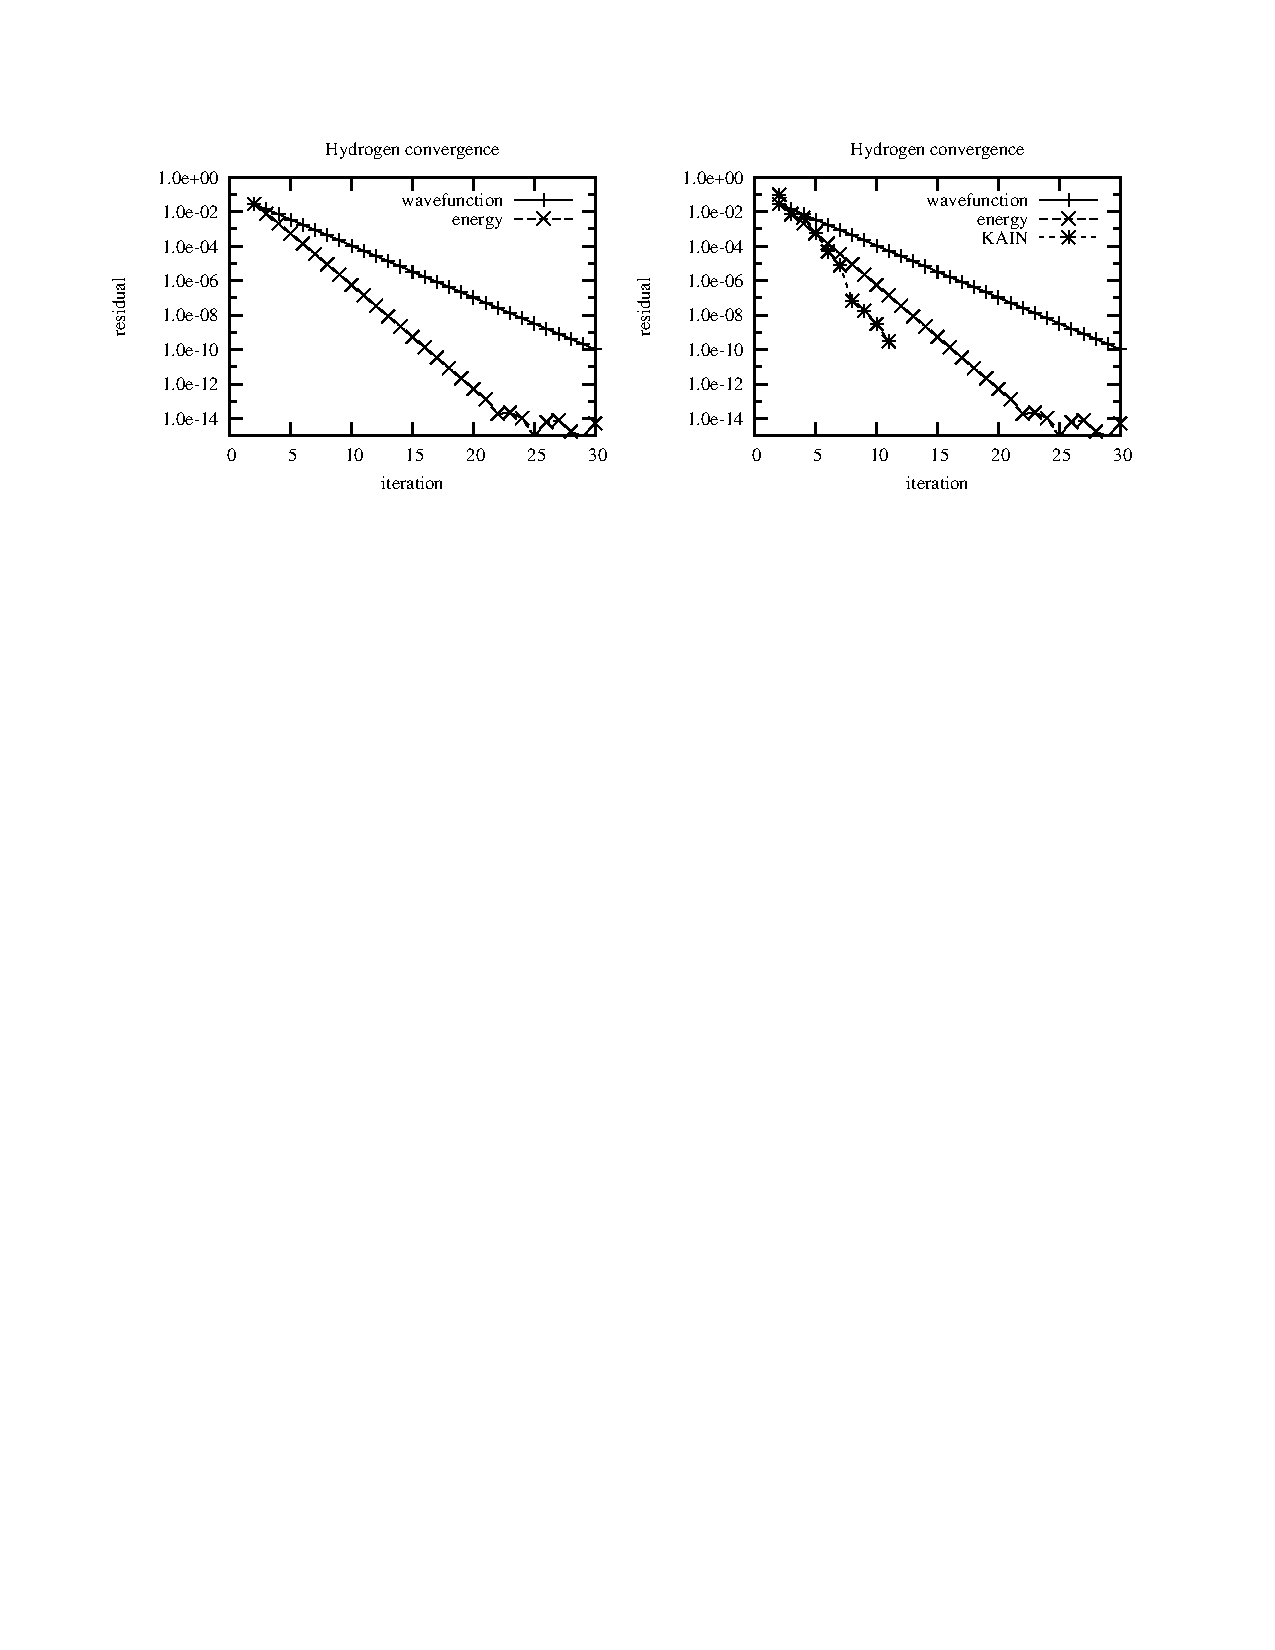
\includegraphics[scale=1.0, clip, viewport = 50 550 300 730]{figures/h_convergence.pdf}
%   \end{center}
% \end{frame}

\begin{frame}
  \frametitle{Hydrogen atom}

  Traditional:
  \begin{itemize}
    \item Algebraic problem that is an approximation (projection) to the physical model
    \item Virtual contributions rotated into occupied space
    \item Finding exact solution to this approximate problem (constraints of fixed basis)
    \item No update to the potential - solution found in single iteration
  \end{itemize}

  MWs:
  \begin{itemize}
    \item Not a fixed basis, no virtual orbitals
    \item Need to "sample" virtual space by application of BSH Green's function
    \item Finding approximate solution to exact numerical problem
    \item We still need to iterate with a \emph{fixed} external potential
  \end{itemize}
\end{frame}

% \begin{frame}
%     \frametitle{Krylov subspace Accelerated Inexact Newton (KAIN)}
%     \begin{columns}
%     \begin{column}[b]{0.5\textwidth}
%     \centering
%     \textbf{Wavefunction history}
%     \begin{equation}
% 	\nonumber
% 	\psi^0, \psi^1, \dots, \psi^n
%     \end{equation}
%     \end{column}
%     \begin{column}[b]{0.5\textwidth}
%     \centering
%     \textbf{Residual history}
%     \begin{equation}
% 	\nonumber
% 	f(\psi^0), f(\psi^1), \dots, f(\psi^n)
%     \end{equation}
%     \end{column}
%     \end{columns}
%
%     \vspace{5mm}
%
%     \centering
%     \textbf{Used to find a better approximation to the Jacobian}
%
%     \vspace{10mm}
%
%     The new iterative step is then expanded in the Krylov subspace
%     \begin{equation}
% 	\nonumber
% 	\delta\psi^n = \sum_i c_i\Big(\psi^i-\psi^n\Big) -
% 	\sum_i c_i\Big(f(\psi^i) - f(\psi^n)\Big) - f(\psi^n)
%     \end{equation}
%
%     \vspace{5mm}
%
%     by solving the linear system $Ac = b$
%     \begin{align}
% 	\nonumber
% 	A_{ij} &= \langle\psi^n-\psi^i|f(\psi^n) - f(\psi^j)\rangle\\
% 	\nonumber
% 	b_{i}  &= \langle\psi^n-\psi^i|f(\psi^n)\rangle
%     \end{align}
%
%     \vspace{5mm}
%
%     \centering
%     \tiny
%     RJ Harrison,
%     {\it J. Comput. Chem.},
%     \textbf{25(3)},
%     328 (2004)
% \end{frame}
%
% \begin{frame}
%     \frametitle{One-electron algorithm}
%
%     \begin{columns}
%     \begin{column}{.50\textwidth}
%     \centering
%     \textbf{Initialize BSH operator} $\hat{G}^n$
%     \begin{equation}
%         \nonumber
%         \mu^n = \sqrt{-2E^n}
%     \end{equation}
%     \end{column}
%
%     \begin{column}{.50\textwidth}
%     \centering
%     \textbf{Power iteration}
%     \begin{equation}
% 	\nonumber
% 	\tilde{\psi}^{n+1} = -2\hat{G}^n \Big[ \hat{V} \psi^n \Big]
%     \end{equation}
%     \end{column}
%     \end{columns}
%
%     \vspace{5mm}
%
%     \begin{columns}
%     \begin{column}{.50\textwidth}
%     \centering
%     \textbf{Wavefunction update}
%     \begin{equation}
% 	\nonumber
% 	\Delta\psi^n = \frac{\tilde{\psi}^{n+1}}{\|\tilde{\psi}^{n+1}\|} - \psi^n
%     \end{equation}
%     \end{column}
%
%     \begin{column}{.50\textwidth}
%     \centering
%     \textbf{Energy update}
%     \begin{equation}
% 	\nonumber
% 	\Delta E^n =
%         \frac{\langle\tilde{\psi}^{n+1}|\hat{V}|\Delta\tilde{\psi}^n\rangle}
%         {\langle\tilde{\psi}^{n+1}|\tilde{\psi}^{n+1}\rangle}
%     \end{equation}
%     \end{column}
%     \end{columns}
%
%     \vspace{5mm}
%
%     \centering
%     \textbf{KAIN update}
%     \begin{equation}
% 	\nonumber
%         \left(
%         \begin{matrix}
%         \delta \psi\\
%         \delta E
%         \end{matrix}
%         \right)^{n+1}
%         \longleftarrow
%         \left(
%         \begin{matrix}
%         \psi\\
%         E
%         \end{matrix}
%         \right)^n
%         ,
%         \left(
%         \begin{matrix}
%         \Delta \psi\\
%         \Delta E
%         \end{matrix}
%         \right)^n
%     \end{equation}
%
%     \vspace{5mm}
%
%     \textbf{Update wavefunction and energy}
%     \begin{align}
% 	\nonumber
%         \psi^{n+1}  &= \psi^n + \delta \psi^n\\
% 	\nonumber
%         E^{n+1}     &= E^n + \delta E^n
%     \end{align}
% \end{frame}
%
% \begin{frame}
%     \frametitle{Hydrogen atom}
%     \begin{center}
% 	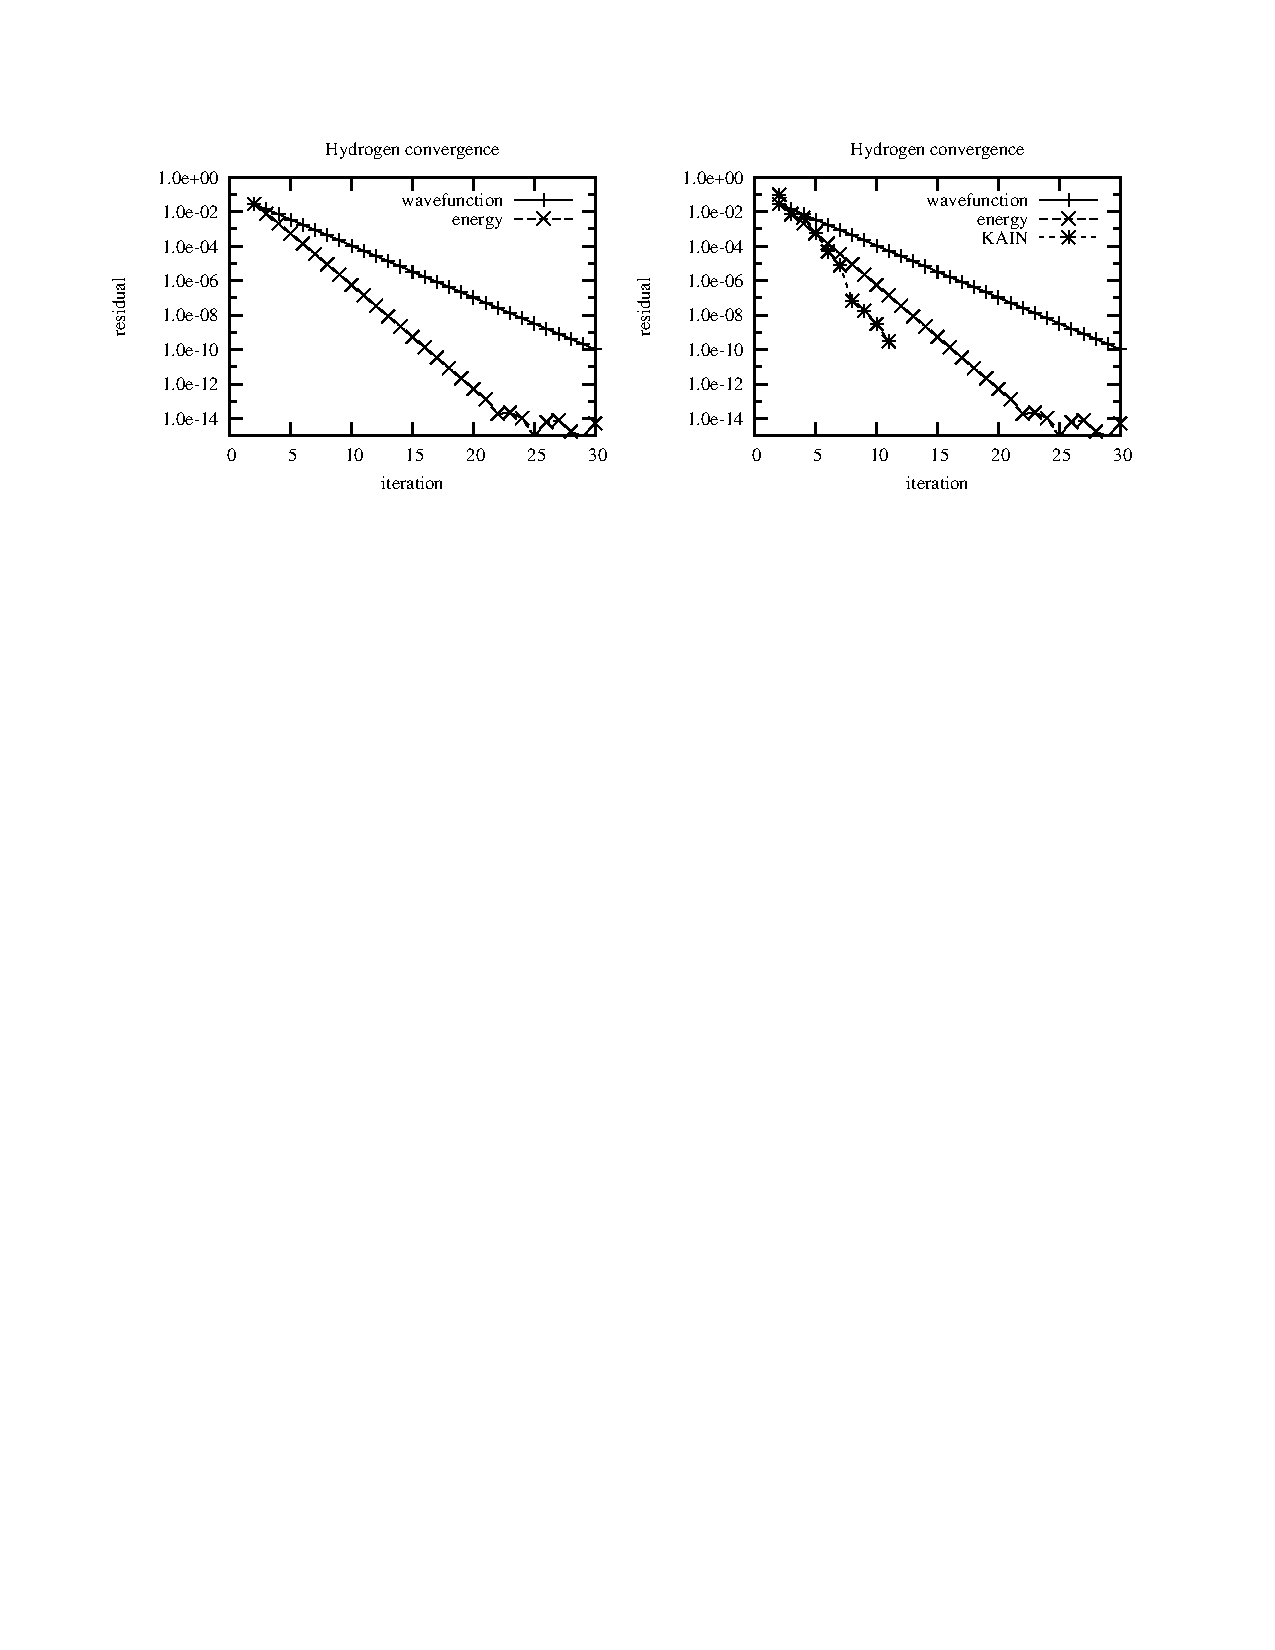
\includegraphics[scale=1.0, clip, viewport = 300 550 560 740]{figures/h_convergence.pdf}
%     \end{center}
% \end{frame}

\begin{frame}
  \frametitle{SCF methods}
  \centering
  \textbf{Potential operator} $0 \leq \alpha \leq 1$
  \begin{equation}
    \nonumber
    \potential = \nucPot(r) + \elPot(r) + \xcPot(r) - \alpha\exchange
  \end{equation}

  \vspace{10mm}

  \begin{columns}
    \begin{column}[b]{0.5\textwidth}
      \centering
      \textbf{Classical nuclear}
      \begin{equation}
        \nonumber
	    \nucPot(r) = -\sum_I\frac{Z_I}{|r-R_I|}
      \end{equation}
    \end{column}

    \begin{column}[b]{0.5\textwidth}
      \centering
      \textbf{Classical Coulomb}
      \begin{equation}
        \nonumber
        \elPot(r) = \int \frac{\density(r')}{|r-r'|} \ud r'
      \end{equation}
    \end{column}
  \end{columns}

  \vspace{5mm}

  \begin{columns}
    \begin{column}[b]{0.5\textwidth}
      \centering
      \textbf{Exchange-Correlation}
      \begin{equation}
        \nonumber
        \xcPot(r)
        = \frac{\delta E_{xc}}{\delta \rho}
        = \frac{\partial F_{xc}}{\partial \density} - \nabla \cdot \frac{\partial F_{xc}}{\partial \nabla\density}
      \end{equation}
    \end{column}

    \begin{column}[b]{0.5\textwidth}
      \centering
      \textbf{Hartree-Fock exchange}
      \begin{equation}
        \nonumber
        \exchange\orbital_p(r) = \sum_i \orbital_i(r) \int \frac{\orbital_i^\dagger(r')\orbital_p(r')}{4\pi|r-r'|} \ud r'
      \end{equation}
    \end{column}
  \end{columns}
\end{frame}

% \begin{frame}
%     \frametitle{Orthonormalization}
%     \centering
%     \textbf{Straightforward iteration of the Kohn-Sham equations}
%     \begin{equation}
%         \nonumber
%         \tilde{\phi}_i^{n+1} = -2\hat{G}_i^n \bigg[\hat{V}^n\phi_i^n\bigg]
%     \end{equation}
%     \textbf{brings all orbitals to the lowest energy eigenfunction}
%
%     \vspace{15mm}
%
%     \textbf{Orthonormality must be imposed}
%     \begin{equation}
%         \nonumber
%         \tilde{S}_{ij} = \langle\tilde{\phi}_i|\tilde{\phi}_j\rangle = \delta_{ij}
%     \end{equation}
%
%     \vspace{5mm}
%
%     \begin{columns}
%     \begin{column}[b]{0.5\linewidth}
%     \centering
%     \textbf{Gram-Schmidt}
%     \begin{equation}
% 	\nonumber
% 	\phi_i = \Big(1 - \sum_{j<i}|\phi_j\rangle\langle\phi_j|\Big)\tilde{\phi}_i
%     \end{equation}
%     \end{column}
%
%     \begin{column}[b]{0.5\linewidth}
%     \centering
%     \textbf{L\"{o}wdin orthonormalization}
%     \begin{equation}
% 	\nonumber
% 	\phi_i = \sum_j \tilde{S}_{ij}^{-1/2}\tilde{\phi}_j
%     \end{equation}
%     \end{column}
%     \end{columns}
% \end{frame}
%
% \begin{frame}
%     \frametitle{Non-canonical orbitals}
%     \centering
%     \textbf{The non-canonical Kohn-Sham equations}
%     \begin{equation}
%         \nonumber
%         \hat{F}|\phi_i\rangle
%         = \bigg[\sum_j|\phi_j\rangle\langle\phi_j|\bigg]\hat{F}|\phi_i\rangle
%         = \sum_jF_{ji}|\phi_j\rangle
%     \end{equation}
%
%     \vspace{5mm}
%
%     \textbf{Rewrite using} $\mu_i^2 = -2\lambda_i$
%     \begin{align}
%         \nonumber
%         \bigg[-\frac{1}{2}\nabla^2 + \hat{V}\bigg]\phi_i
%         &= \sum_jF_{ji}\phi_j\\
%         \nonumber
%         \bigg[-\nabla^2 + \mu_i^2\bigg]\phi_i
%         &= -2\bigg[\hat{V}\phi_i - \sum_j\big(F_{ji} -
%         \lambda_i\delta_{ji}\big)\phi_j\bigg]\\
%         \nonumber
%         \phi_i
%         &= -2\hat{G}_i\bigg[\hat{V}\phi_i - \sum_j\big(F_{ji} -
%         \Lambda_{ji}\big)\phi_j\bigg]
%     \end{align}
%
%     \vspace{5mm}
%
%     \begin{columns}
%     \begin{column}[b]{0.48\linewidth}
%     \centering
%     \textbf{Fock matrix}
%     \begin{equation}
%         \nonumber
%         F_{ij} = \langle\phi_i|\hat{T} + \hat{V}|\phi_j\rangle
%     \end{equation}
%     \end{column}
%
%     \begin{column}[b]{0.48\linewidth}
%     \centering
%     \textbf{Kinetic matrix}
%     \begin{equation}
%         \nonumber
%         T_{ij}
%         = \langle\phi_i|\hat{T}|\phi_j\rangle
%         = \frac{1}{2}\langle\nabla\phi_i|\nabla\phi_j\rangle
%     \end{equation}
%     \end{column}
%     \end{columns}
% \end{frame}
%
% \begin{frame}
%     \frametitle{Localized orbitals}
%     \centering
%     Total energy invariant under unitary transformations among occupied orbitals
%     \begin{equation}
% 	\nonumber
% 	\phi_i = \sum_j L_{ij} \phi_i, \qquad \qquad L^\ast L = LL^\ast = I
%     \end{equation}
%
%     \begin{columns}
%     \begin{column}[b]{0.48\linewidth}
%     \centering
%     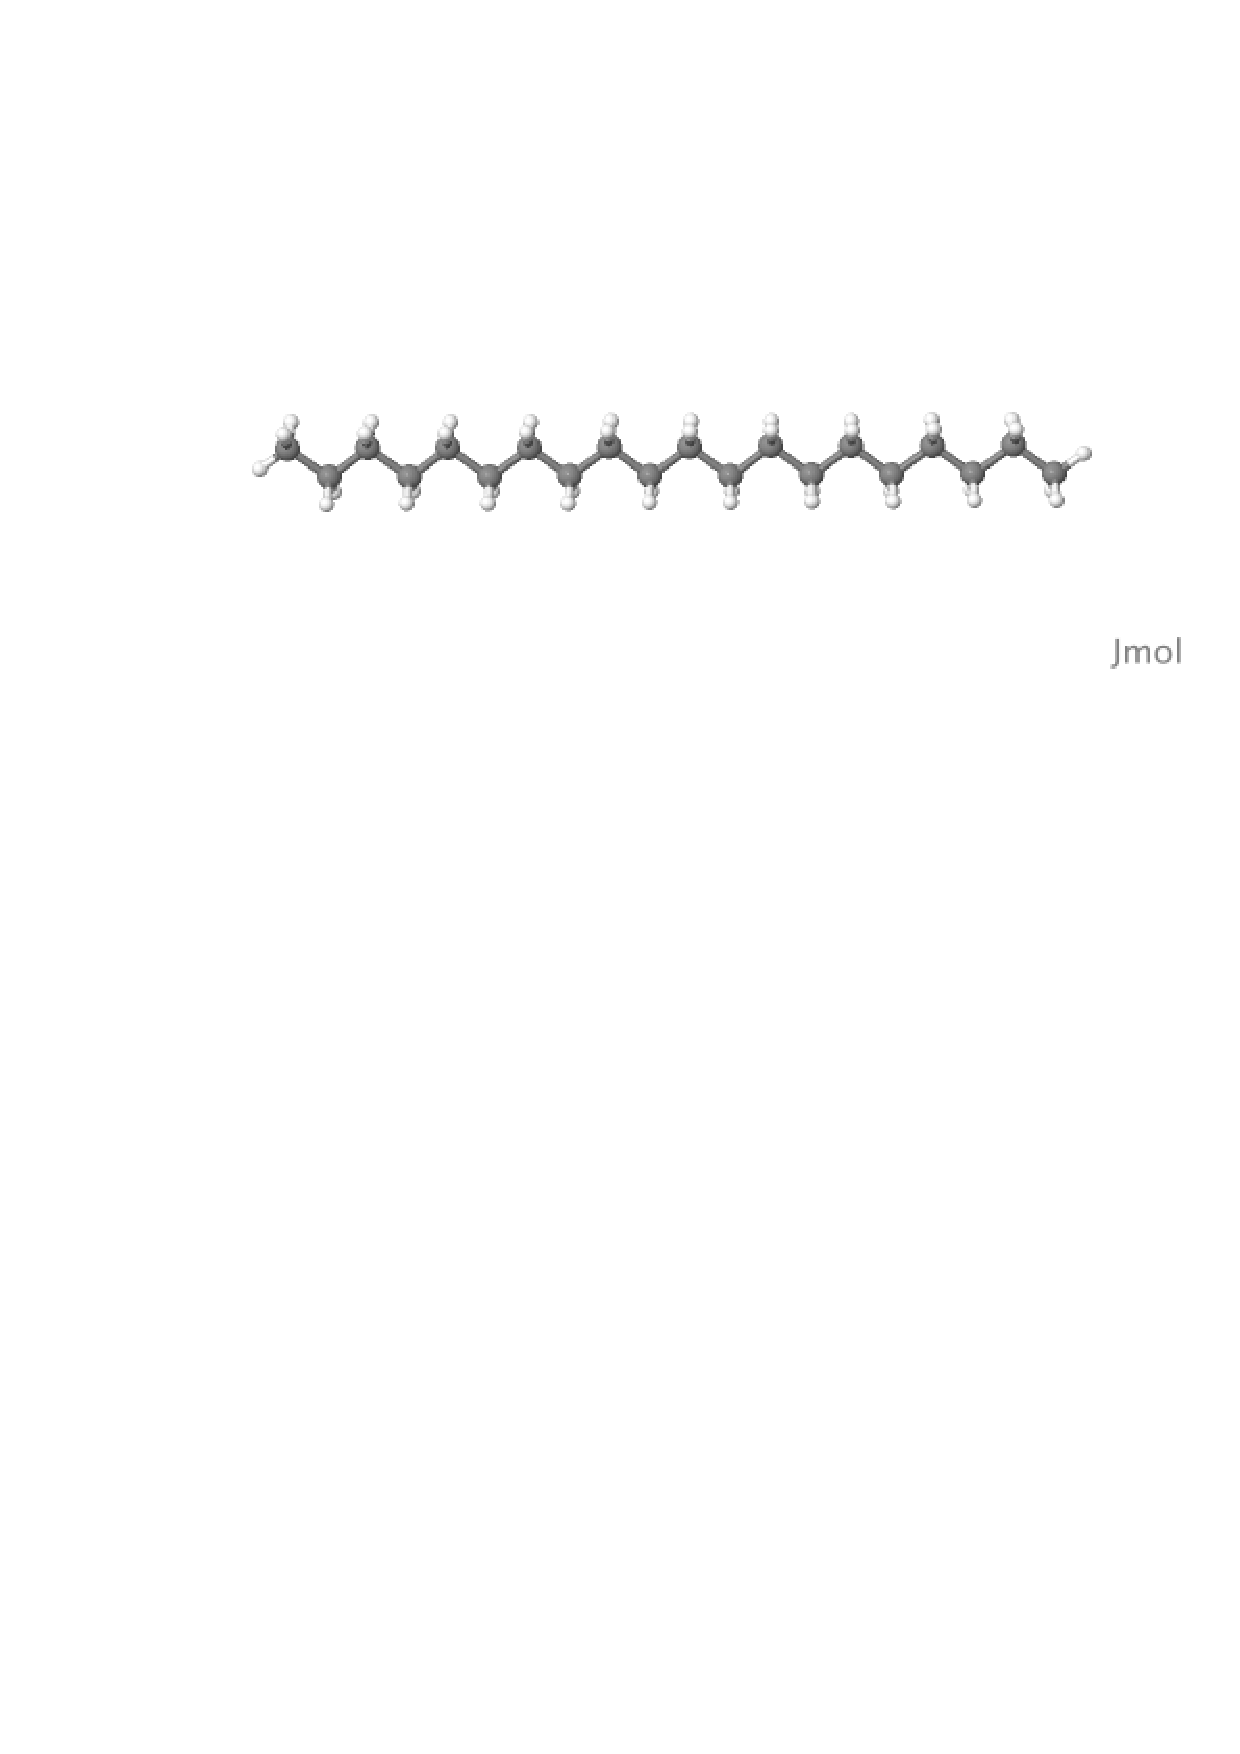
\includegraphics[scale=0.25, clip, viewport = 80 560 600 700]{figures/alkane.pdf}\\
%     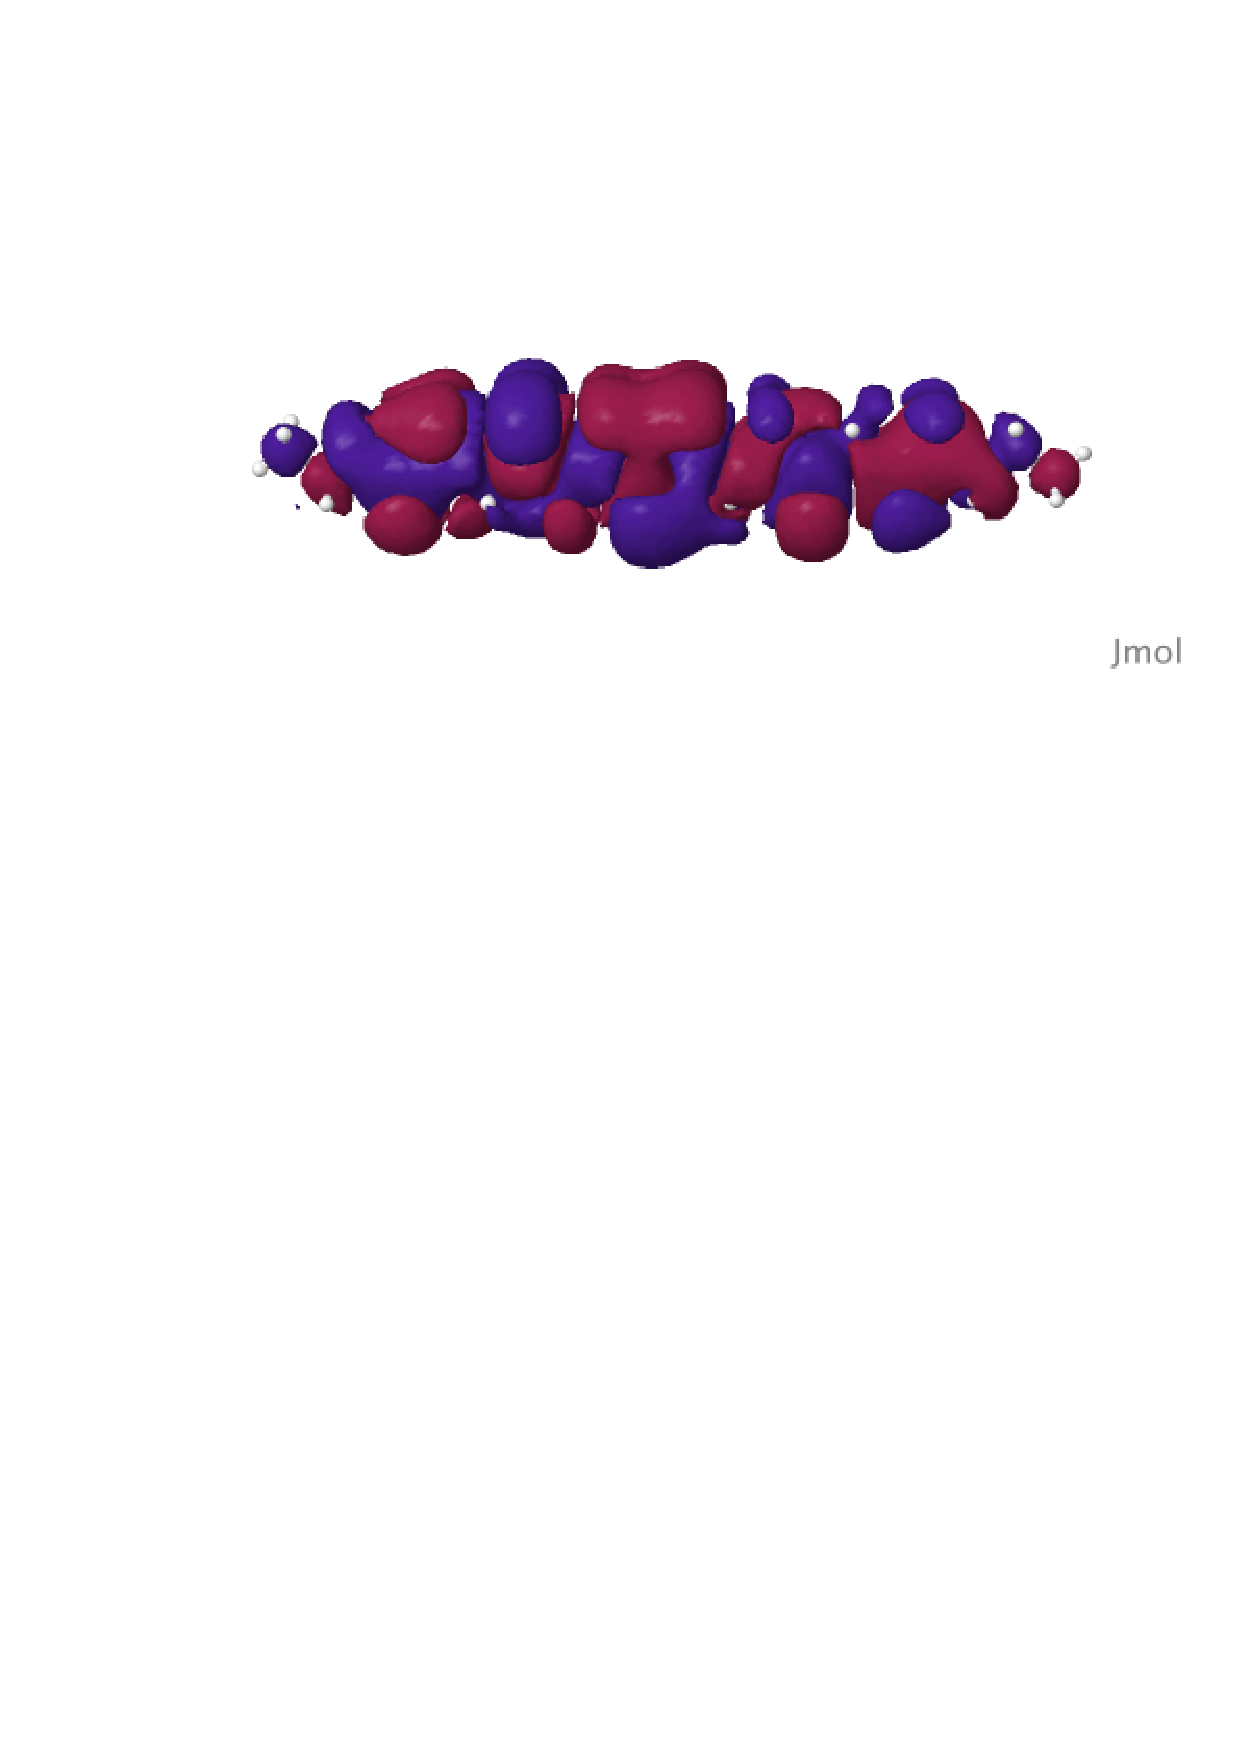
\includegraphics[scale=0.25, clip, viewport = 80 560 600 700]{figures/can_orb_1.pdf}\\
%     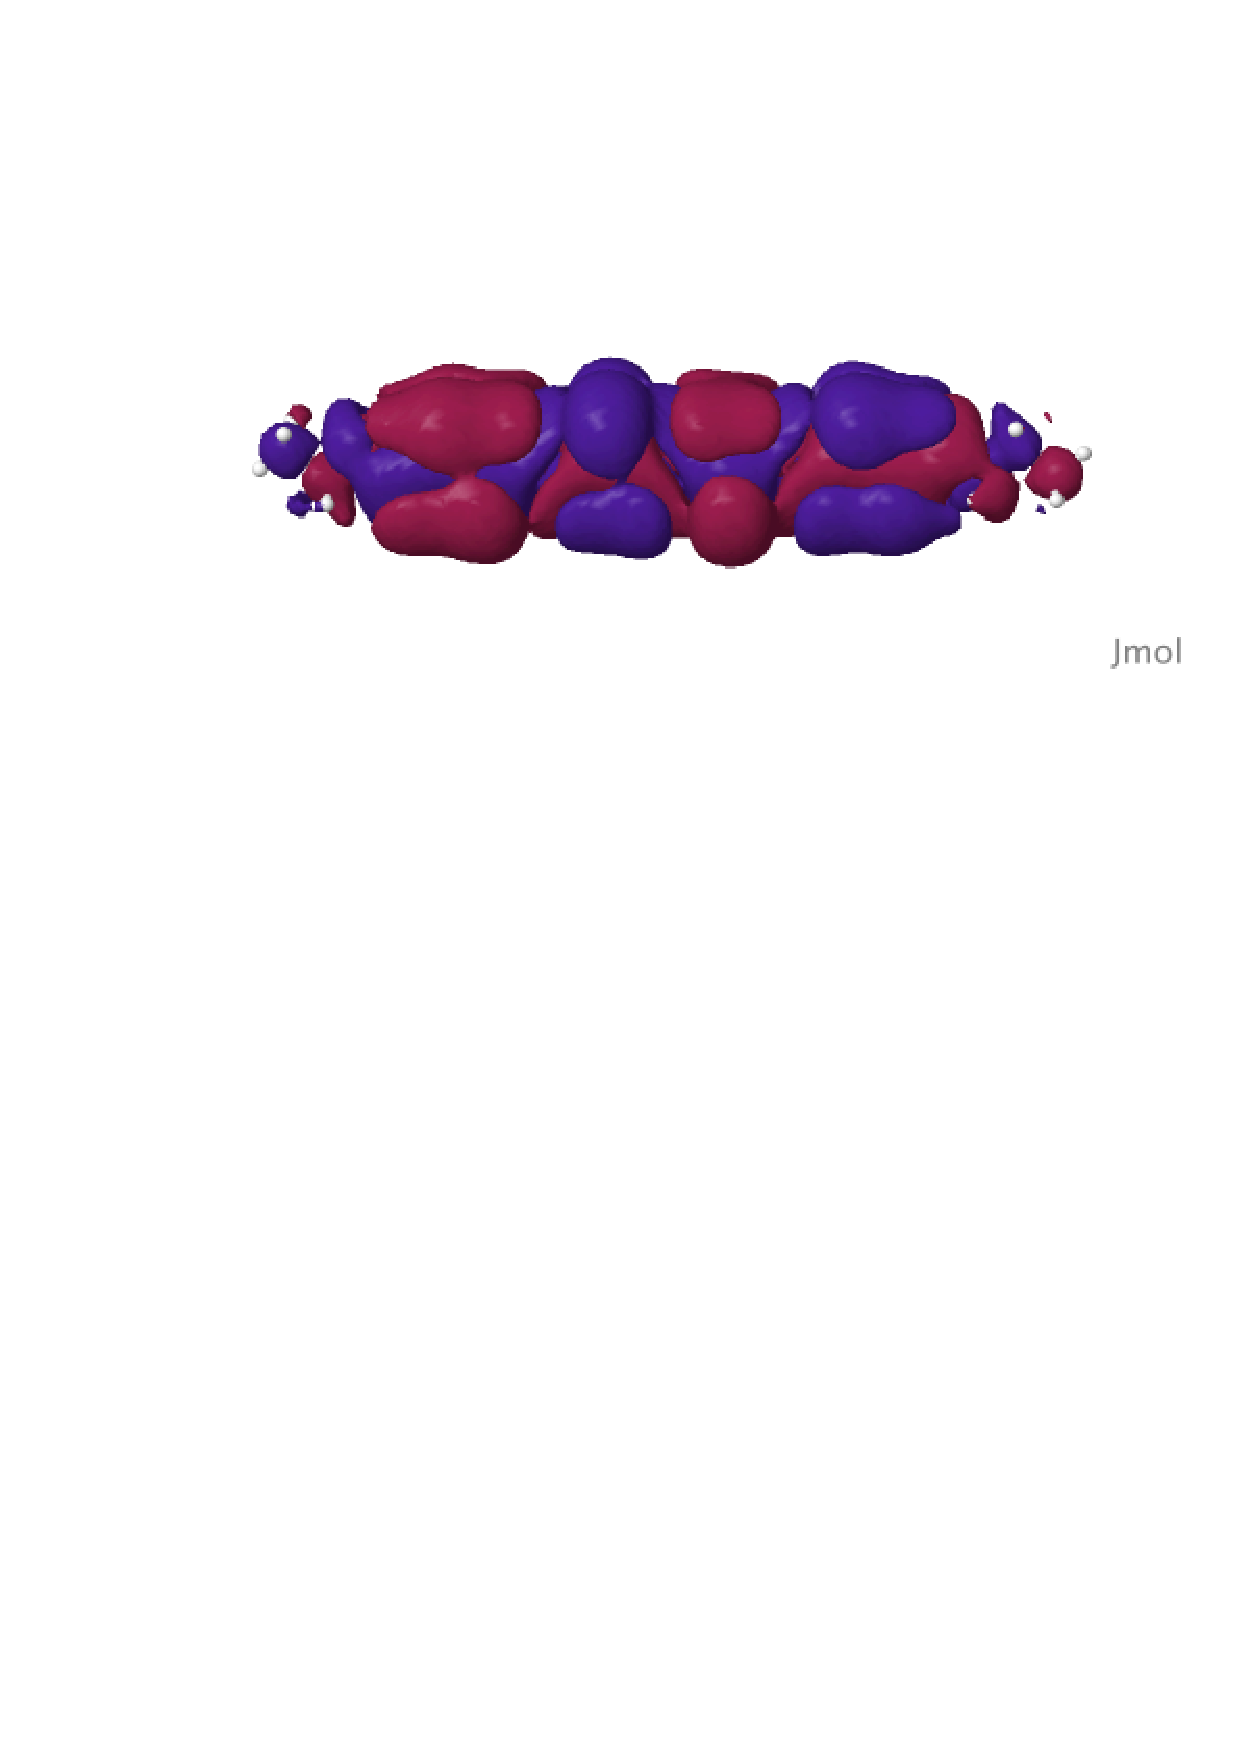
\includegraphics[scale=0.25, clip, viewport = 80 560 600 700]{figures/can_orb_2.pdf}\\
%
%     \vspace{2mm}
%
%     \begin{equation}
%         \nonumber
%         \phi_i =\ -2\hat{G}_i\Bigg[\hat{V}\phi_i
%         - (\epsilon_i - \lambda_i)\phi_i\Bigg]
%     \end{equation}
%     \end{column}
%
%     \begin{column}[b]{0.48\linewidth}
% \only<2>{
%     \centering
%     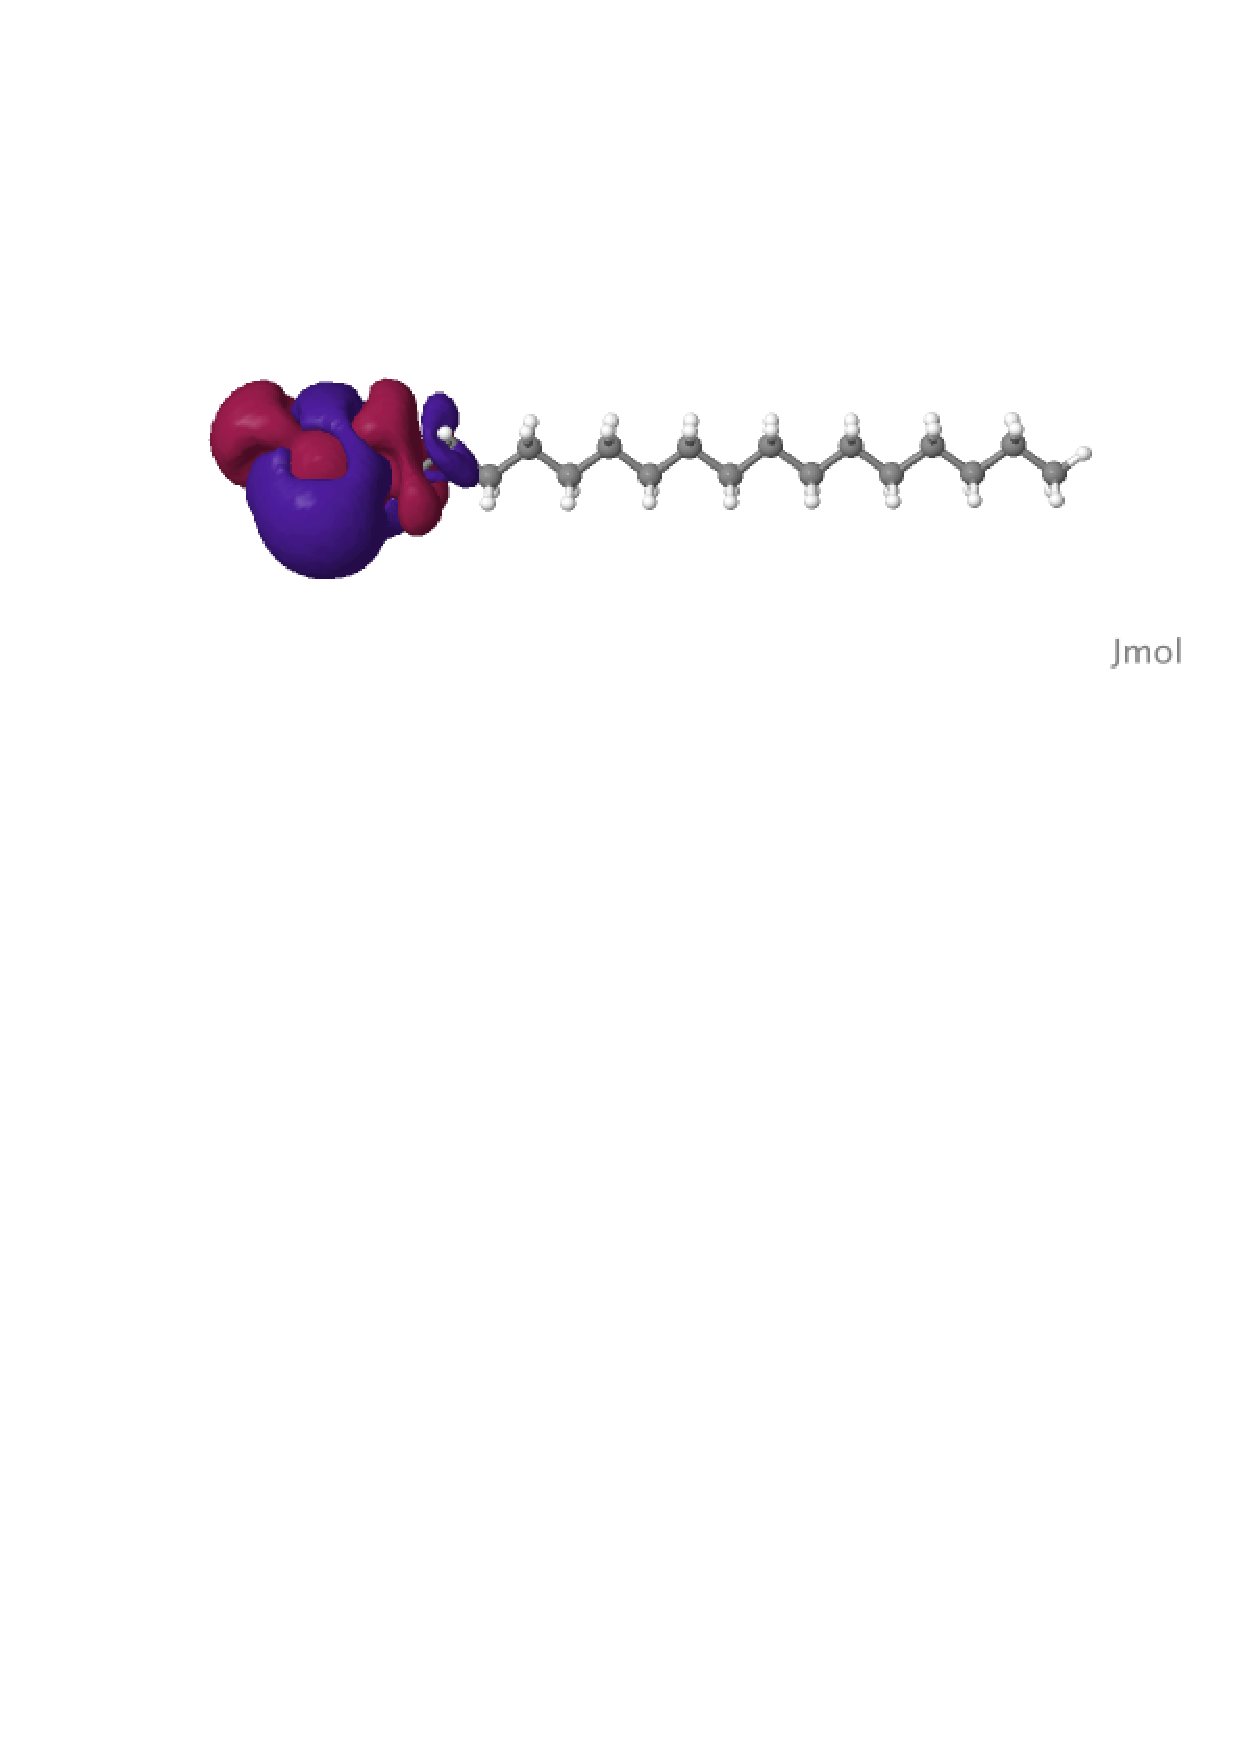
\includegraphics[scale=0.25, clip, viewport = 80 560 600 700]{figures/loc_orb_1.pdf}\\
%     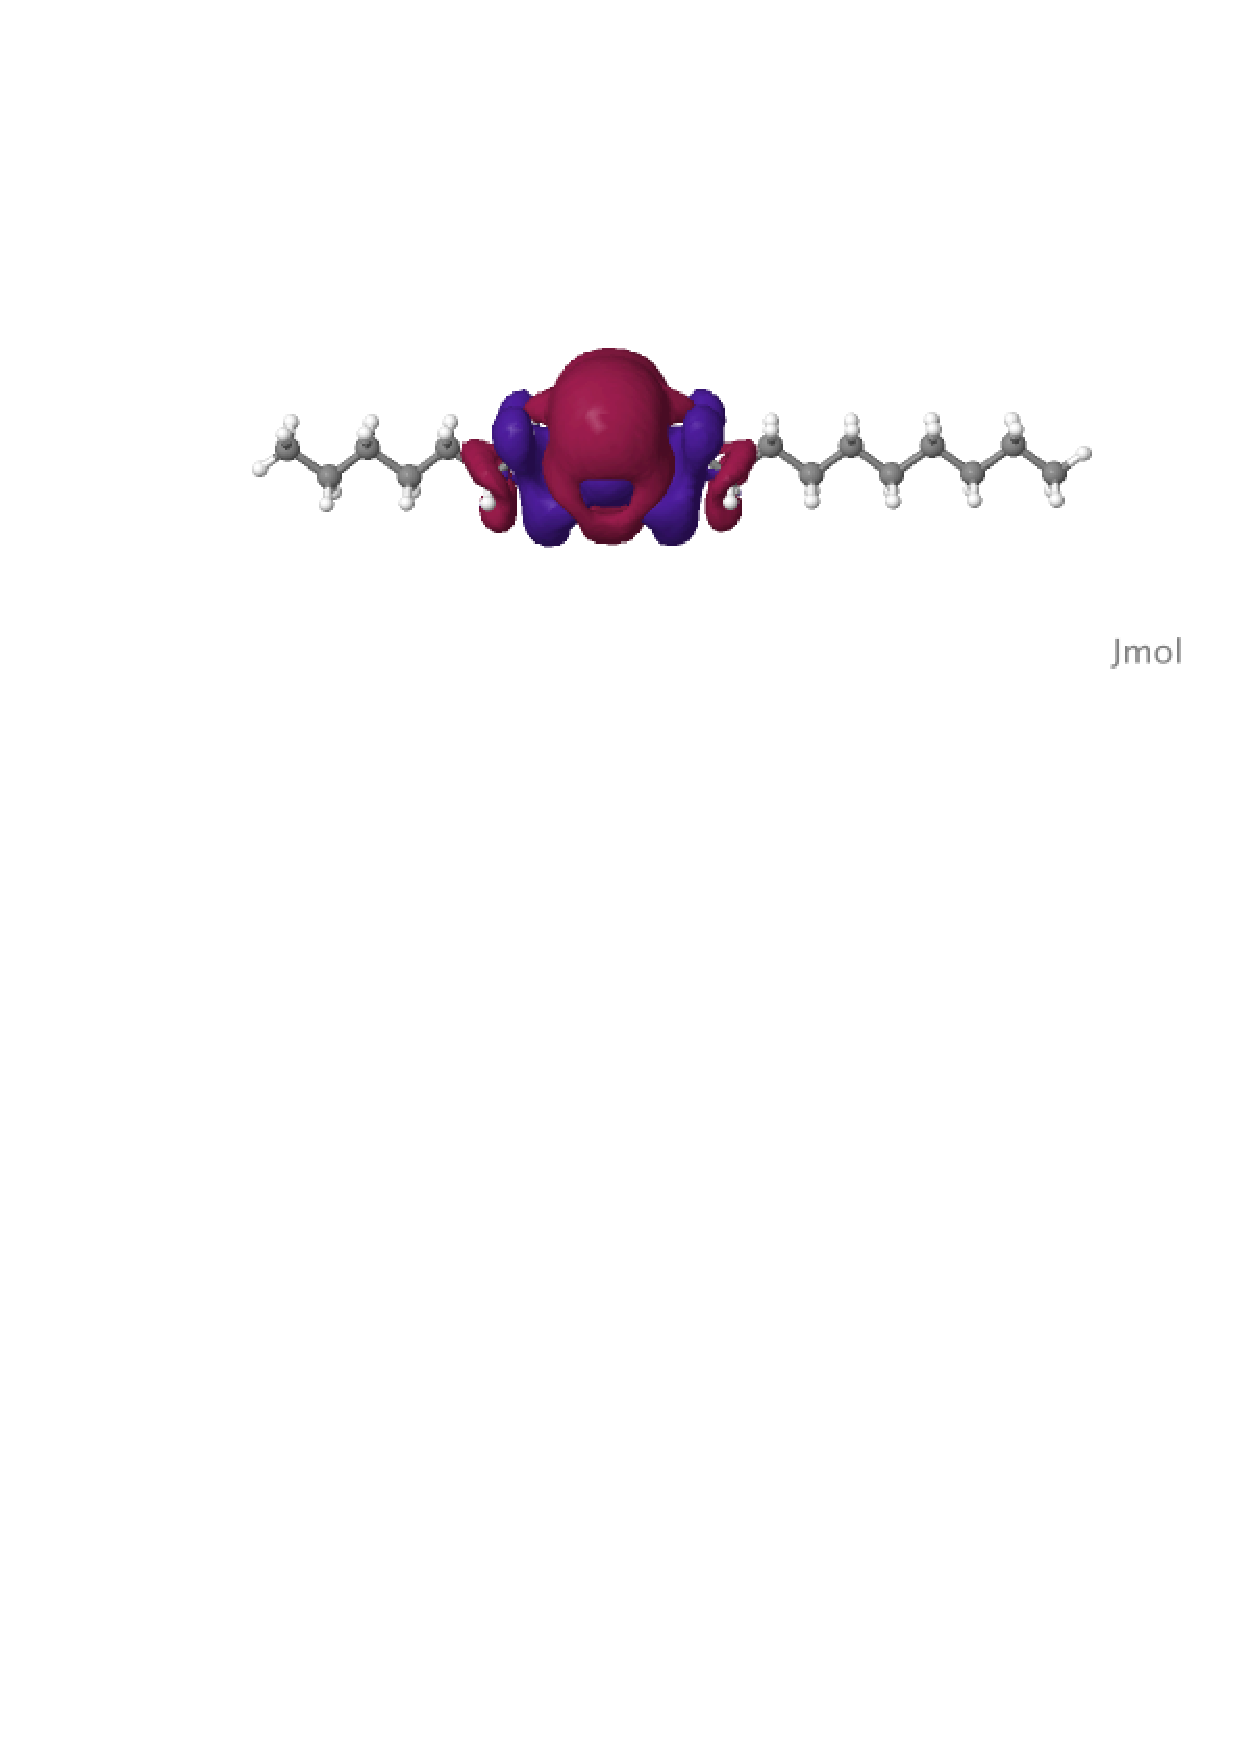
\includegraphics[scale=0.25, clip, viewport = 80 560 600 700]{figures/loc_orb_2.pdf}\\
%     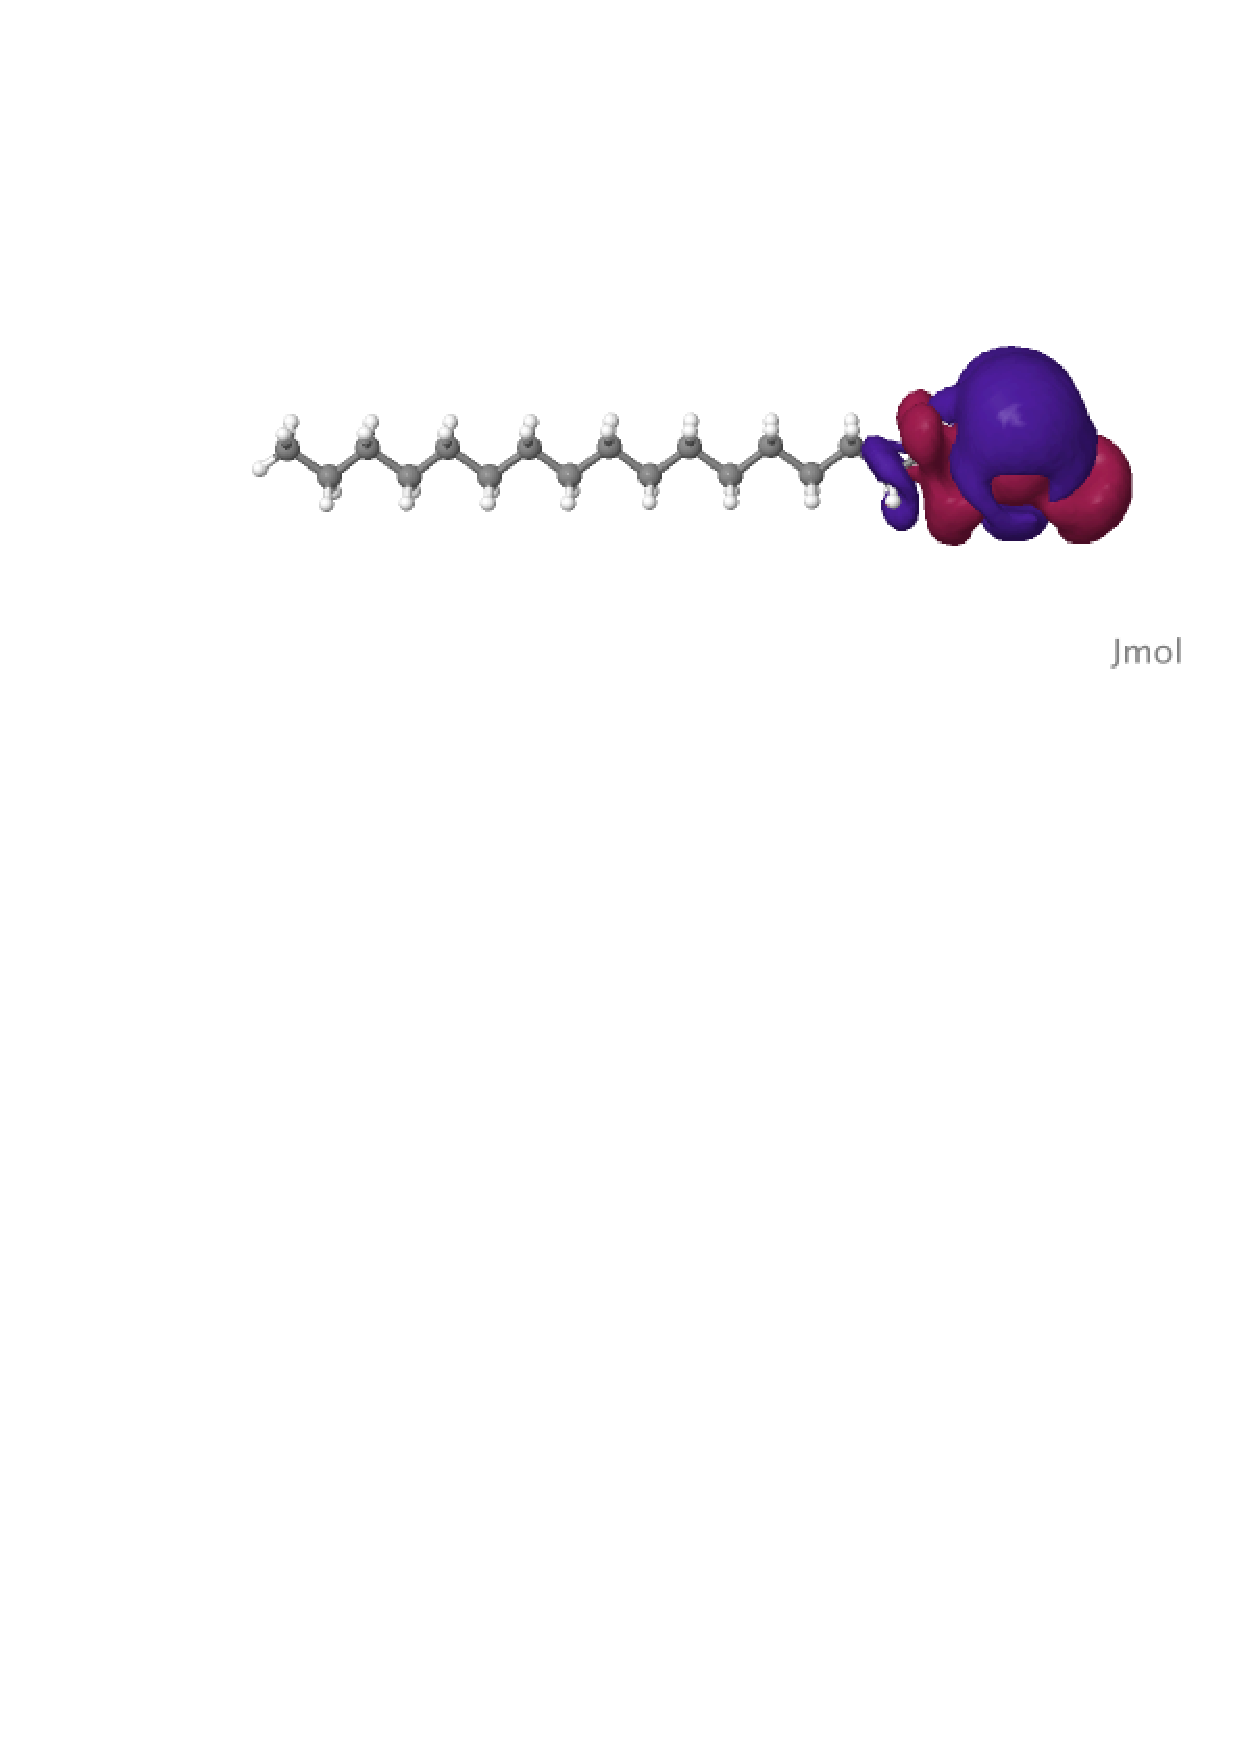
\includegraphics[scale=0.25, clip, viewport = 80 560 600 700]{figures/loc_orb_3.pdf}\\
%
%     \vspace{2mm}
%
%     \begin{equation}
%         \nonumber
%         \phi_i =\ -2\hat{G}_i\Bigg[\hat{V}\phi_i
%         - \sum_j(F_{ji} - \Lambda_{ji})\phi_j\Bigg]
%     \end{equation}
% }
%     \end{column}
%     \end{columns}
%
%     \vspace{6mm}
%
%     \centering
%     \tiny
%     S.F. Boys,
%     {\it Rev. Mod. Phys.},
%     \textbf{32:296}
%     (1960)\\
%     J.M. Foster, S.F. Boys,
%     {\it Rev. Mod. Phys.},
%     \textbf{32:300}
%     (1960)
% \end{frame}

%\begin{frame}
%    \frametitle{Orthonormalization}
%    \centering
%    \textbf{The non-canonical Kohn-Sham equations}
%    \begin{equation}
%        \nonumber
%        \tilde{\phi}_i^{n+1} = -2\hat{G}_i^n \bigg[\hat{V}^n\phi_i^n -
%        \sum_j\big(F_{ji}^n - \Lambda_{ji}^n\big)\phi_j^n\bigg]
%    \end{equation}
%
%    \vspace{10mm}
%
%    \textbf{Overlap matrix}
%    \begin{equation}
%        \nonumber
%        \tilde{S}_{ij} = \langle\tilde{\phi}_i|\tilde{\phi}_j\rangle
%    \end{equation}
%
%    \vspace{10mm}
%
%    \begin{columns}
%    \begin{column}[b]{0.3\linewidth}
%    \centering
%    \textbf{Diagonalize}
%    \begin{equation}
%	\nonumber
%        U = D\tilde{S}^{-1/2}
%    \end{equation}
%    \end{column}
%
%    \begin{column}[b]{0.4\linewidth}
%    \centering
%    \textbf{Localize}
%    \begin{equation}
%	\nonumber
%        U = L\tilde{S}^{-1/2}
%    \end{equation}
%    \end{column}
%
%    \begin{column}[b]{0.3\linewidth}
%    \centering
%    \textbf{Orthonormalize}
%    \begin{equation}
%	\nonumber
%        U = \tilde{S}^{-1/2}
%    \end{equation}
%    \end{column}
%    \end{columns}
%
%    \vspace{10mm}
%
%    \centering
%    \textbf{Orbital rotation}
%    \begin{equation}
%	\nonumber
%	\phi_i = \sum_j U_{ij} \tilde{\phi}_j \qquad \qquad F = U\tilde{F}U^{-1}
%    \end{equation}
%\end{frame}

% \begin{frame}
%     \frametitle{Many-electron algorithm I}
%     \centering
%     \textbf{Setup Fock operator} $\hat{F}^n$
%
%     \vspace{5mm}
%
%     \textbf{Compute Fock matrix} $F_{ij}^n = \langle\phi_i^n|\hat{F}^n|\phi_j^n\rangle$
%
%     \vspace{5mm}
%
%     \textbf{Diagonalize/Localize}
%
%     \vspace{5mm}
%
%     \textbf{Iterate BSH operators with} $\lambda_i^n \approx F_{ii}^n$
%     \begin{equation}
% 	\nonumber
%         \tilde{\phi}_i^{n+1} = -2\hat{G}_i^n \bigg[\hat{V}^n\phi_i^n -
%         \sum_j\big(F_{ji}^n - \Lambda_{ji}^n\big)\phi_j^n\bigg]
%     \end{equation}
%
%     \vspace{2mm}
%
%     \textbf{Orthonormalize} $S^{-1/2}$
%
%     \vspace{5mm}
%
%     \textbf{Compute KAIN update} $\delta\phi_i^n$
%
%     \vspace{5mm}
%
%     \textbf{Orthonormalize} $S^{-1/2}$
%
% \end{frame}
%
% \begin{frame}
%     \frametitle{Many-electron algorithm I}
%     \centering
%     \textbf{Overall accuracy kept at} $\epsilon = 10^{-6}$
%     \begin{center}
% 	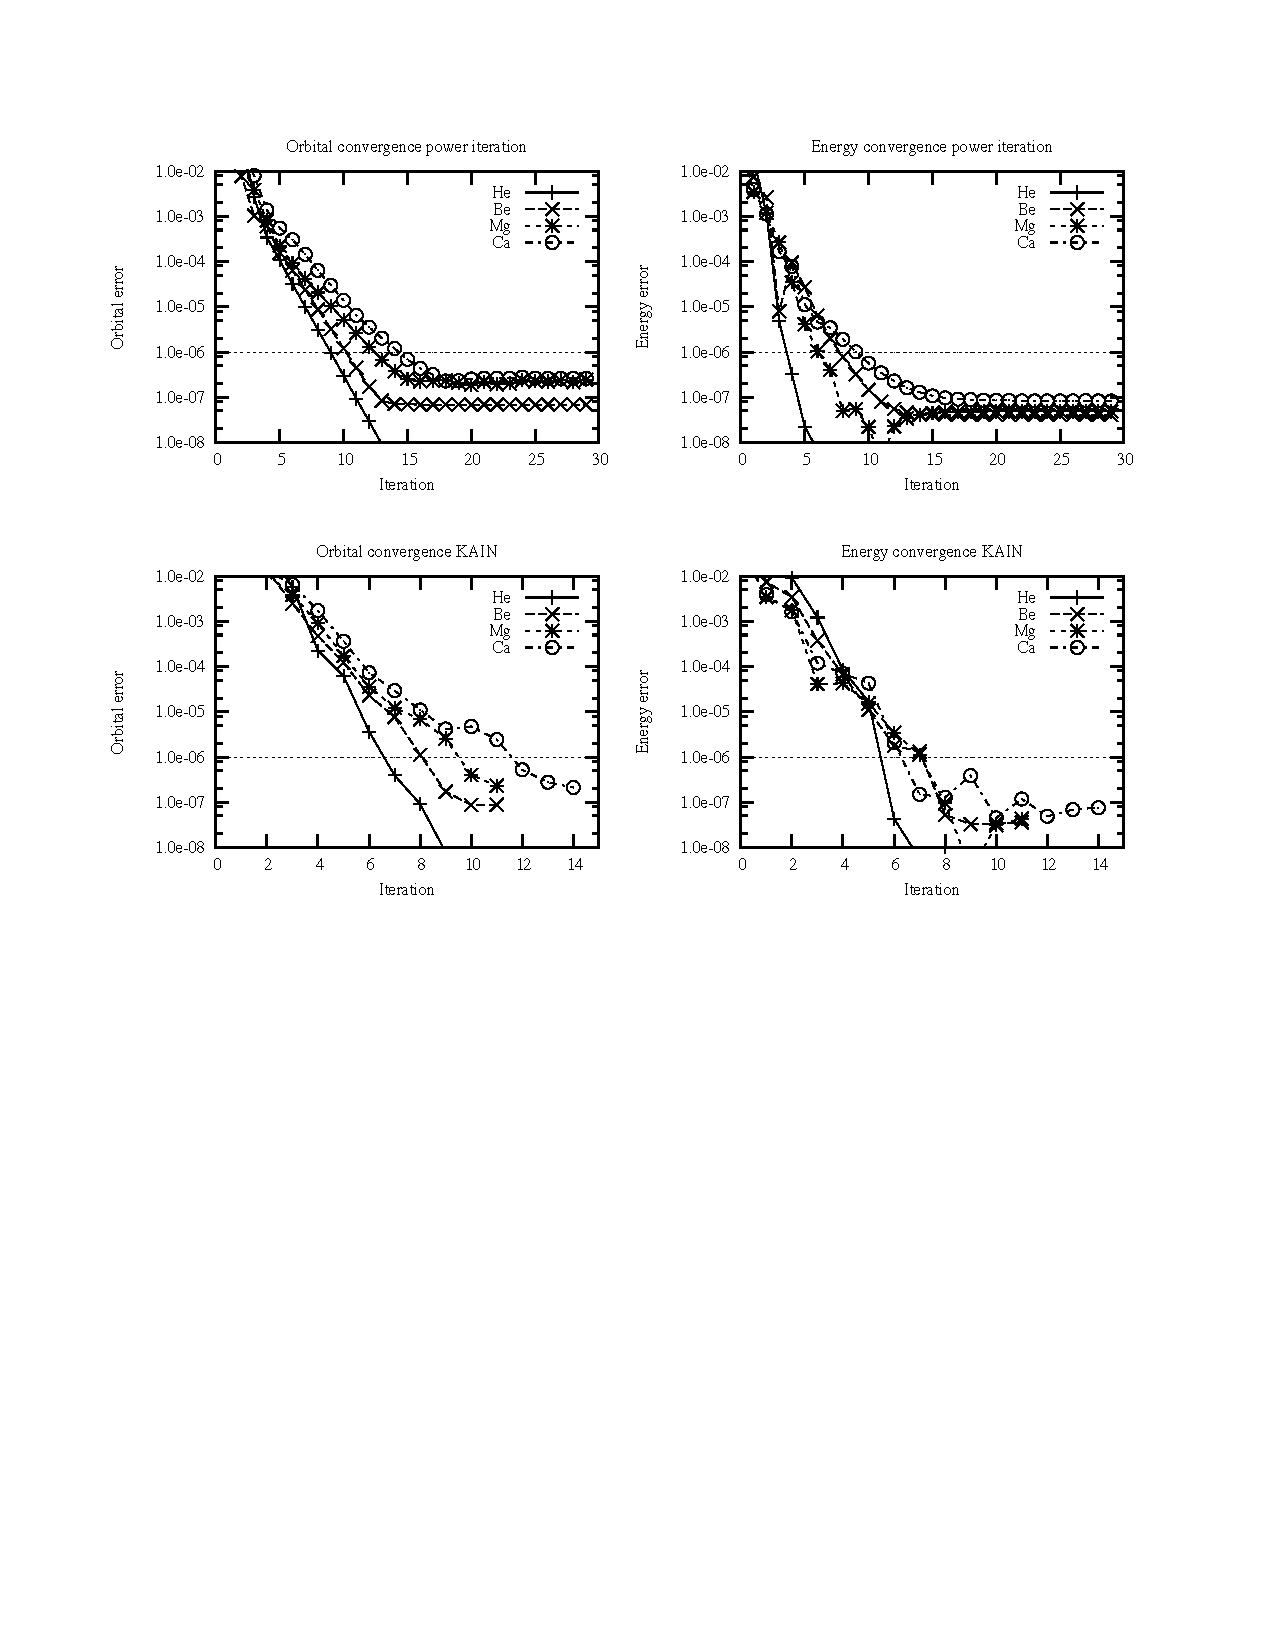
\includegraphics[scale=1.0, clip, viewport = 50 550 300 740]{figures/accuracy.pdf}
%     \end{center}
% \end{frame}
%
% \begin{frame}
%     \frametitle{Many-electron algorithm I}
%     \begin{columns}
%     \begin{column}[b]{0.70\linewidth}
%         \centering
%         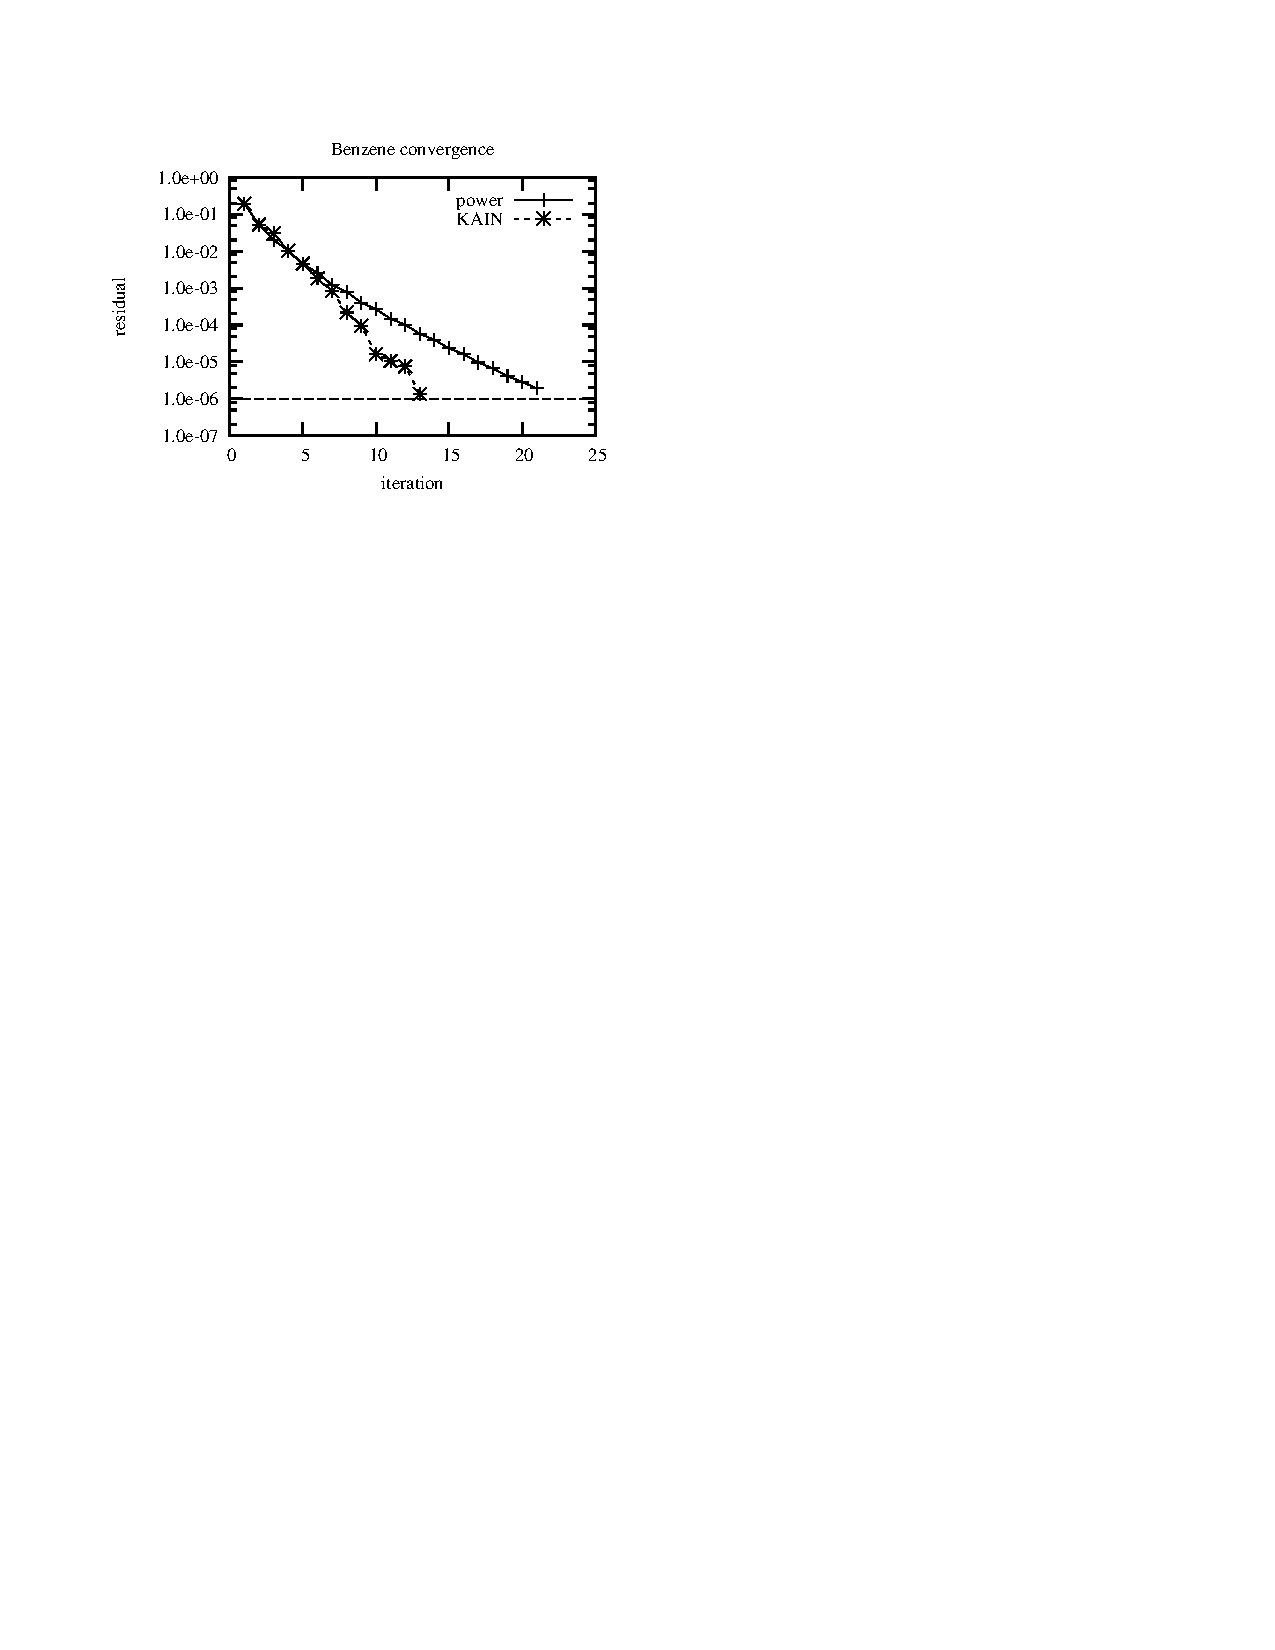
\includegraphics[scale=0.8, clip, viewport = 50 550 300 730]{figures/benzene_convergence.pdf}
%     \end{column}
%     \begin{column}[b]{0.30\linewidth}
%         \centering
%         \textbf{Benzene}
%         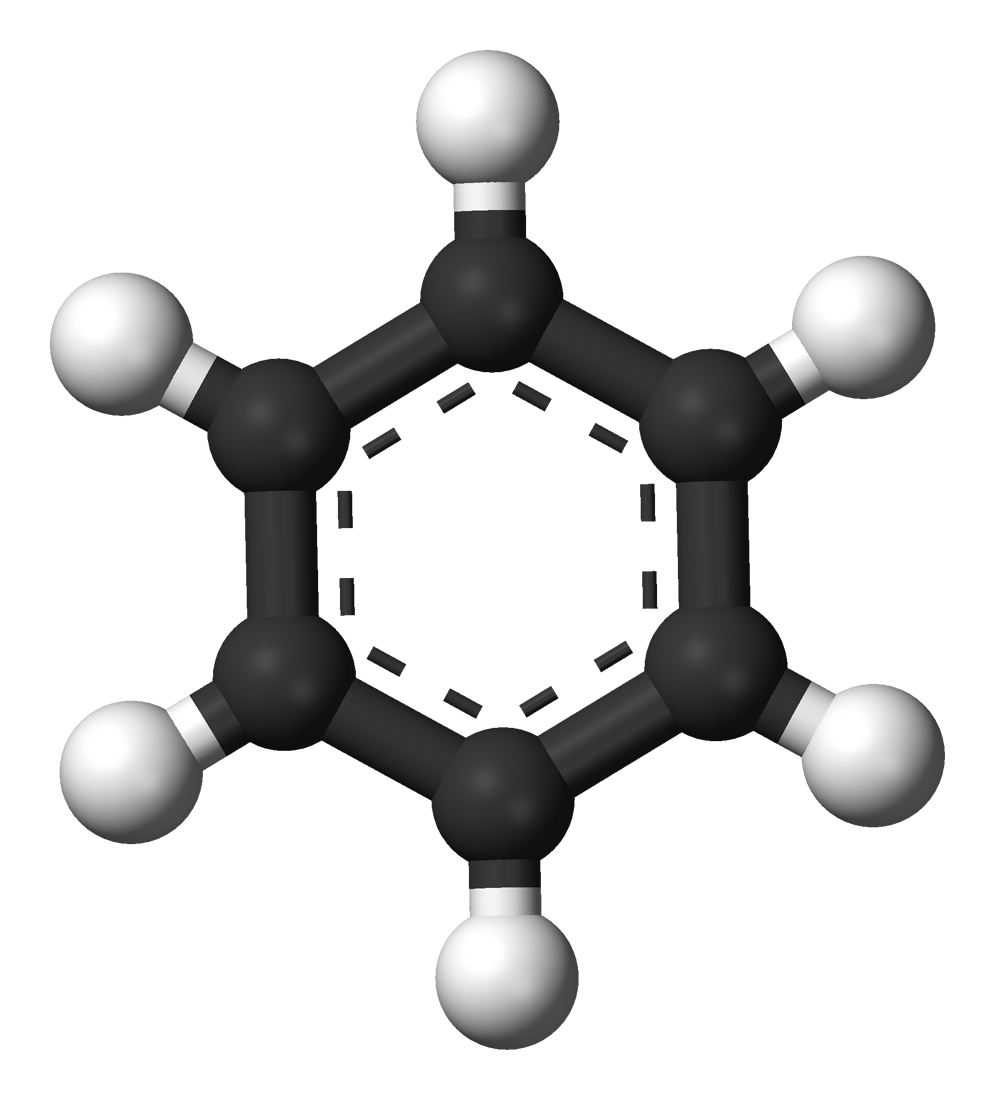
\includegraphics[scale=0.1, clip, viewport = 0 0 1000 1200]{figures/benzene.png}
%
%         \vspace{5mm}
%
%     \end{column}
%     \end{columns}
% \end{frame}
%
% \begin{frame}
%     \frametitle{Many-electron algorithm II}
%     \centering
%     \textbf{Setup Fock operator} $\hat{F}^n$
%
%     \vspace{8mm}
%
%     \textbf{Iterate BSH operators with} $\lambda_i^n \approx F_{ii}^n$
%     \begin{equation}
% 	\nonumber
%         \tilde{\phi}_i^{n+1} = -2\hat{G}_i^n \bigg[\hat{V}^n\phi_i^n -
%         \sum_j\big(F_{ji}^n - \Lambda_{ji}^n\big)\phi_j^n\bigg]
%     \end{equation}
%
%     \vspace{2mm}
%
%     \textbf{Compute potential updates} $\Delta\hat{V}^n$
%
%     \vspace{8mm}
%
%     \textbf{Update Fock matrix}
%     \begin{equation}
%         \nonumber
%         \tilde{F}^{n+1} = F^{n} +
%         \Delta \tilde{S}_1^n F^n +
%         \Delta \tilde{S}_2^n \Lambda^n +
%         \Delta \tilde{F}_{pot}^n
%     \end{equation}
%
%     \vspace{5mm}
%
%     \textbf{Orthonormalize} $\tilde{S}^{-1/2}$
%
%     \vspace{5mm}
%
%     \textbf{Diagonalize/localize}
%
% \end{frame}

%\begin{frame}
%    \frametitle{Total energy calculation}
%    \centering
%    \textbf{Kohn-Sham energy expression}
%    \begin{equation}
%        \nonumber
%        E[\rho] = T_s[\rho] + V_{en}[\rho] + J[\rho] + E_{xc}[\rho]
%    \end{equation}
%
%    \vspace{3mm}
%
%    \textbf{Closed-shell system}
%    \begin{equation}
%        \nonumber
%        E = \sum_i^{N/2} 2\langle \orbital_i|\hat{T}|\orbital_i \rangle
%	    + \int \rho(r)v_{nuc}(r) \ud r
%	    + \frac{1}{2} \int \rho(r)v_{el}(r) \ud r
%	    + \int F_{xc} \ud r
%    \end{equation}
%
%    \vspace{3mm}
%
%    \textbf{Sum of orbital energies}
%    \begin{equation}
%        \nonumber
%        \sum_i^{N/2} 2\epsilon_i
%	    = \sum_i^{N/2} 2\langle\orbital_i|\hat{T} + \hat{V}|\orbital_i\rangle
%	    = \sum_i^{N/2} 2\langle\orbital_i|\hat{T}|\orbital_i\rangle
%	        + \int \rho(r)\Big[v_{nuc}(r)+v_{el}(r)+v_{xc}(r)\Big] \ud r
%    \end{equation}
%
%    \vspace{3mm}
%
%    \textbf{Alternative expression}
%    \begin{equation}
%        \nonumber
%        E = 2 \sum_i^{N/2} \epsilon_i - \frac{1}{2} \int \rho(r)v_{el}(r) \ud r
%	    + \int F_{xc} \ud r - \int \rho(r)v_{xc}(r) \ud r
%    \end{equation}
%\end{frame}
